\documentclass[chaptersright]{informeutn}
% con la opcion chaptersright los capitulos empiezan siempre en pagina impar

\usepackage{circuitikz}
\usepackage{amsmath}
\usepackage{float}
\usepackage{mathrsfs}
\usepackage{colortbl}
\usepackage{multirow}
\usepackage{pgfplots}
\pgfplotsset{compat=1.18}

\materia{An\'alisis de Se\~nales y Sistemas}
\titulo{Trabajo Práctico 2}
\comision{2R1}
\autores{Ernst Pedro 400624\\Leiva Matias 92170\\Tissera Mauro 401187\\Perea Ignacio 406265}
\fecha{17 / 08 / 2025}

\begin{document}

\maketitle

\tableofcontents
\setcounter{page}{1}
\thispagestyle{plain}

\chapter{Ejercicio 1}

\section{Actividad 1}

\textbf{Actividad 1}. Dada la secuencia de senales {$\phi_{n} (t)=e^{j(n\omega)t}: n \in \mathbb{Z}$}, con $T = \dfrac{2\pi}{\omega}$. Demostrar:

\subsection{A}

\textbf{A)} El periodo fundamental de la senal $\phi_{n}(t)$ es $T_n=\dfrac{2\pi}{n\omega}$. ¿Por qué se puede afirmar que la suma entre estas señales está bien definida $\phi_{n}(t)$?

\textbf{i.} Lo primero que realizaremos seria corroborar que $T_n$ es un periodo.

$$\phi_{n}(t+T_n)=\phi_{n}(t)$$

$$e^{jn\omega(t+T_n)}=e^{jn\omega(t)}$$

$$e^{jn\omega(t+\dfrac{2\pi}{n\omega})}=e^{jn\omega(t)}$$

$$e^{jn\omega(t)+jn\omega\dfrac{2\pi}{n\omega}}=e^{jn\omega(t)}$$

$$e^{jn\omega(t)+j2\pi}=e^{jn\omega(t)}$$

$$e^{jn\omega(t)} \cdot e^{j2\pi} = e^{jn\omega(t)}$$

$$e^{jn\omega(t)} \cdot 1 = e^{jn\omega(t)}$$

$$e^{jn\omega(t)} = e^{jn\omega(t)}$$

\textbf{ii.} Para ver que $T_n$ es el periodo fundamental, suponemos que exisite un $T'>0$ con $T'<T_n$, tal que.

$$\phi_n(t+T')=\phi_n(t)$$

Entonces $e^{jn\omega T'} = 1$, por lo que existe $k \in \mathbb{Z}$ tal que

$$n\omega T'= 2\pi k$$

Despejando $n\omega$

$$T'=\dfrac{2\pi k}{n\omega}$$

Donde si $k=0$ entonces $T'=0$, lo cual contradic lo que postulamos al principio que $T'>0$

Si $|k| \ge 1$, entonces

$$T' \ge \dfrac{2\pi}{|n|\omega} = T_{|n|}$$

Lo cual contradice que $T'<T_n$. Por lo tanto no existe $T'\in(0,T_n)$ que sea periodo.

\textbf{iii.}

Ahora bien podemos concluir que la suma $\sum_{n \in \mathbb{Z}} \phi_n(t)$ está bien definida porque todas las señales $\phi_n(t)$ son periódicas con un periodo común $T = \frac{2\pi}{\omega}$ (múltiplo entero de $T_n$). Esto garantiza que la superposición de señales mantenga la periodicidad global.

\vspace{0.5cm}

\subsection{B}

\textbf{B)} Calcular $E_n = (\phi_n(t), \phi_n(t))_T \quad \text{y} \quad (\phi_n(t), \phi_m(t))_T, \quad \forall n,m \in \mathbb{Z}$

Como primer paso definiremos
\[
\langle \phi_n, \phi_m \rangle_T = \frac{1}{T}\int_0^T \phi_n(t)\overline{\phi_m(t)}dt
\]

\textbf{Caso 1: $n = m$}
\begin{align*}
\langle \phi_n, \phi_n \rangle_T &= \frac{1}{T}\int_0^T e^{jn\omega t}e^{-jn\omega t}dt \\
&= \frac{1}{T}\int_0^T 1\,dt = 1 \quad \forall n
\end{align*}

\textbf{Caso 2: $n \neq m$}
\begin{align*}
\langle \phi_n, \phi_m \rangle_T &= \frac{1}{T}\int_0^T e^{j(n-m)\omega t}dt \\
&= \left.\frac{e^{j(n-m)\omega t}}{j(n-m)\omega T}\right|_0^T = 0 \quad \text{(por periodicidad)}
\end{align*}

\vspace{0.5cm}

\subsection{C}

\textbf{C)} La secuencia de señales $\{ \phi_n(t) = e^{j(n\omega)t} : n \in \mathbb{Z} \}$ es base de Fourier.

\textbf{Propiedades requeridas:}
\begin{enumerate}[label=(\roman*)]
\item \textbf{Ortogonalidad}: $\langle \phi_n, \phi_m \rangle_T = \delta_{nm}$ (demostrado en B)
\item \textbf{Completitud}: Cualquier señal $x(t)$ periódica puede expresarse como:
\[
x(t) = \sum_{n=-\infty}^{\infty} C_n \phi_n(t)
\]
\end{enumerate}

\vspace{0.5cm}

\subsection{D}

\textbf{D)} La secuencia de señales $\{ \rho_n^0(t) = \cos(n\omega t) = \tfrac{1}{2}\phi_n(t) + \tfrac{1}{2}\overline{\phi_n(t)} : n \geq 0 \}$ es base de Fourier.

\textbf{Relación con $\phi_n(t)$:}
\[
\cos(n\omega t) = \frac{1}{2}\phi_n(t) + \frac{1}{2}\phi_{-n}(t)
\]

\textbf{Ortogonalidad:}
\[
\langle \rho_n^0, \rho_m^0 \rangle_T = 
\begin{cases}
1 & n = m = 0 \\
\frac{1}{2} & n = m \neq 0 \\
0 & n \neq m
\end{cases}
\]

\vspace{0.5cm}

\subsection{E}

\textbf{E)} La secuencia de señales \[\{ \rho_n^1(t) = \sin(n\omega t) = \tfrac{1}{2j}\phi_n(t) - \tfrac{1}{2j}\overline{\phi_n(t)} : n > 0 \}\] es base de Fourier.

\textbf{Relación con $\phi_n(t)$:}
\[
\sin(n\omega t) = \frac{1}{2j}\phi_n(t) - \frac{1}{2j}\phi_{-n}(t)
\]

\textbf{Ortogonalidad:}
\[
\langle \rho_n^1, \rho_m^1 \rangle_T = 
\begin{cases}
\frac{1}{2} & n = m \\
0 & n \neq m
\end{cases}
\]

\section{Actividad 2}

\textbf{Actividad 2.} Calcular la descomposicion de series $x(t) = \sum_{n \in \mathbb{Z}}$ y $x(t) = a_0 + \sum_{n=1}^{\infty}(a_n \rho_n ^0(t) + b_n \rho_n ^1(t))$ de las siguientes se\~nales. Para luego calcular aproximadamente la energia de la se\~nal usando el teorema de Parseval.

\subsection{Se\~nal sinusoidal rectificada de onda completa}

\begin{figure}[H]
  \centering
  \includegraphics[width=0.8\textwidth]{photos/onda_completa.png}
\end{figure}

La se\~nal se trata de $x(t) = |sen(t)|$.

Primero debemos tomar el periodo de la se\~nal, el cual es igual a $\pi$, para poder calcular el coeficiente $C_n$ el cual esta dado por la siguiente ecuacion.

$$C_n = \dfrac{1}{T} \int_{<T>} x(t) e^{-j(n\omega)t} dt$$

$$C_n = \dfrac{1}{\pi} \int_{0}^{\pi} |sen(t)| e^{-j(n\omega)t} dt$$

Siendo $\omega = \dfrac{2\pi}{T} = 2$

Quedando $e^{-j(n\omega)t} = e^{-j2nt} = cos(2nt)-j\,sen(2nt)$

$$C_n = \dfrac{1}{\pi} \int_{0}^{\pi} |sen(t)| [\cos(2nt) - j sen(2nt)] dt$$

$$C_n = \dfrac{1}{\pi} \bigg[\int_{0}^{\pi} sen(t) cos(2nt) dt + j \int_{0}^{\pi} sen(t) sen(2nt) dt \bigg] $$

Siendo $ \int_{0}^{\pi} sen(t) sen(2nt) dt = 0$

$$C_n = \dfrac{1}{\pi} \bigg[\int_{0}^{\pi} sen(t) cos(2nt) dt + 0 \bigg] $$

Recordando que $sen(A) cos(B) = \dfrac{1}{2} [sen(A+B) + sen(A-B)] $

$$C_n = \dfrac{1}{\pi} \int_{0}^{\pi} \dfrac{1}{2} \bigg[sen(t+2nt)+sen(t-2nt)\bigg] dt $$

$$C_n = \dfrac{1}{\pi}  \dfrac{1}{2} \bigg[\int_{0}^{\pi} sen((1+2n)t) dt + \int_{0}^{\pi}sen((1-2n)t) dt\bigg]$$

$$C_n = \dfrac{1}{2\pi} \bigg[\dfrac{-cos((1+2n)\pi)+cos(0)}{1+2n} + \dfrac{-cos((1-2n)\pi)+cos(0)}{1-2n}  \bigg] $$ 

$$C_n = \dfrac{1}{2\pi} \bigg[\dfrac{-(-1)+1}{1+2n} + \dfrac{-(-1)+1}{1-2n} \bigg]  $$

$$C_n = \dfrac{1}{2\pi} \bigg[\dfrac{2}{1+2n} + \dfrac{2}{1-2n} \bigg] $$

$$C_n = \dfrac{1}{2\pi} \bigg[\dfrac{4}{-4n^2+1}\bigg] $$

$$C_n = -\dfrac{2}{\pi(4n^2+1)}$$

Ahora para escribir la serie recordemos que $\phi_n (t) = e^{j(n\omega)t}$.

$$x(t) = \sum_{n \in \mathbb{Z}} C_n \phi_n (t)$$

$$x(t) = \sum_{n=0}^{\infty} \dfrac{-2}{\pi(4n^2+1)} e^{j2nt} $$

$$x(t) = \dfrac{-2}{\pi} \sum_{n=0}^{\infty} \dfrac{e^{j2nt}}{4n^2+1}$$

Si desarrollamos los primeros terminos de la serie queda

$$x(t) = \dfrac{-2}{\pi} \bigg[1 + \dfrac{e^{j2t}}{5} + \dfrac{e^{j4t}}{17} + \dfrac{e^{j6t}}{37} + ... \bigg] $$

Para expresar la se\~nal en su segunda forma (la cual si es posible ya que la se\~nal con la que estamos trabajando SI es real) nos es de suma importancia saber si la se\~nal es tiene simetria, par, impar o no tiene simetria.

Para que sea par debe cumplir con que $f(-t) = f(t)$, veamos.

$$f(-t) = |sen(-t)| = |-sen(t)| = |sen(t)| = f(t) $$

Por lo que verificamos que la se\~nal es par, entonces

$$b_n = 0 $$

$$a_0 = \dfrac{2}{T} \int_{<\dfrac{T}{2}>} x(t) dt $$

$$a_n = \dfrac{4}{T} \int_{<\dfrac{T}{2}>} x(t) cos \bigg(\dfrac{2n\pi t}{T} \bigg) $$

\chapter{Ejercicio 2}

\section{Actividad 1}

\textbf{A)} Expresar la Ecuación Diferencial (ED) que describe el circuito, y con ello, definir un
Sistema en tiempo continuo con entrada x(t) = v(t) y salida y(t) = i(t) , con condiciones
Iniciales genérica (CI).

\begin{figure}[H]
  \centering
  \begin{circuitikz}[american voltages]
    \node at (-3,1) {ENTRADA};
    \node at (-3,0) {$x(t) = v(t)$};
    
    \draw (-1,-1) rectangle (3.5,2.5);

    \draw (-0.5,1.5) to[R=$R$] (2,1.5)
          to[C=$C$] (2,-0.5) -- (-0.5,-0.5);
    
    \draw[->] (-4, 0.5) -- (-1,0.5);

    \node at (6,1) {SALIDA};
    \node at (6,0) {$y(t) = i(t)$};
    
    \draw[->] (3.5,0.5) -- (6,0.5);
  \end{circuitikz}
\end{figure}

Para plantear la EDO es necesario plantear ley de kirchoff

$$v(t) = R \cdot i(t) + \dfrac{1}{C} \cdot \int i(t) dt$$

Ahora derivamos para conseguir la expresion buscada

$$\dfrac{d v(t)}{dt} = R \dfrac{d i(t)}{dt} + \dfrac{1}{C} \cdot i(t)$$

Dividimos todo por $R$ para normalizar la ecuacion

$$\dfrac{d i(t)}{dt} + \dfrac{1}{RC} \cdot i(t) = \dfrac{1}{R} \cdot \dfrac{d v(t)}{dt}$$

$$y'(t) + \dfrac{1}{RC} \cdot y(t) = \dfrac{1}{R} \cdot x'(t)$$

Para el circuito de segundo orden:

\begin{figure}[H]
  \centering
  \begin{circuitikz}[american voltages]
    \node at (-3,1) {ENTRADA};
    \node at (-3,0) {$x(t) = v(t)$};
    
    \draw (-1,-1) rectangle (3.5,2.5);

    \draw (-0.5,1.5) to[R=$R$] (1.25,1.5) to[L=$L$] (2.3,1.5)
          to[C=$C$] (2.3,-0.5) -- (-0.5,-0.5);
    
    \draw[->] (-4, 0.5) -- (-1,0.5);

    \node at (6,1) {SALIDA};
    \node at (6,0) {$y(t) = i(t)$};
    
    \draw[->] (4,0.5) -- (6,0.5);
  \end{circuitikz}
\end{figure}

Siguiendo con el mismo procedimiento

$$v(t) = R \cdot i(t) + L \cdot \dfrac{d i(t)}{dt} + \dfrac{1}{C} \cdot \int i(t) dt$$

$$\dfrac{d v(t)}{dt} = R \cdot \dfrac{d i(t)}{dt} + L \cdot \dfrac{d^2 i(t)}{dt^2} + \dfrac{1}{C} \cdot i(t)$$

$$\dfrac{d^2 i(t)}{dt^2} +  \dfrac{R}{L} \cdot \dfrac{d i(t)}{dt} + \dfrac{1}{LC} \cdot i(t) = \dfrac{1}{L} \cdot \dfrac{d v(t)}{dt} $$

$$y''(t) + \dfrac{R}{L} \cdot y'(t) + \dfrac{1}{LC} \cdot y(t) = \dfrac{1}{L} \cdot x'$$

\textbf{B)}Usar la transformada de Laplace para sintetizar el sistema en la expresión

Primero sintetizamos la ecuacion correspondiente al circuito de primer orden

$$\mathscr{L}[y'(t)] = sY(s) - y(0)$$

$$\mathscr{L}[y(t)] = Y(s)$$

$$\mathscr{L}[x'(t)] = sX(s) - x(0)$$

Quedando la ecuacion

$$sY(s) - y(0) + \dfrac{1}{RC} \cdot Y(s) = \dfrac{1}{R} \cdot (sX(s) - x(0))$$

$$Y(s) (s + \dfrac{1}{rc}) = \dfrac{1}{R} \cdot sX(s) - \dfrac{1}{R} x(0) + y(0)$$

$$Y(s) = X(s)  \dfrac{\dfrac{s}{R}}{s + \dfrac {1}{RC}} + \dfrac{1}{(s + \dfrac{1}{RC})} [y(0) - x(0) \dfrac{1}{R}]$$

Ya nos queda sintetizado a la expresion

$$Y(s) = X(s) \cdot H(s) + F(s,CI)$$

Ahora para el circuito de segundo orden, primero debemos definir la transformada para la segunda derivada

$$\mathscr{L}[y''(t)] = s^2Y(s) - sy(0) - y'(0)$$

Quedando la ecuacion sintetizada

$$ s^2Y(s) - s y(0) - y'(0) + \dfrac{R}{L} (sY(s) - y(0)) + \dfrac{1}{LC} \cdot Y(s) = \dfrac{1}{L} \cdot (sX(s) - x(0))$$

$$ Y(s) (s^2 + \dfrac{R}{L} s + \dfrac{1}{LC}) = X(s) \dfrac{s}{L} - x(0) \dfrac{1}{L} + s y(0) + y'(0) + \dfrac{R}{L} y(0)$$

$$ Y(s) = X(s) \dfrac{\dfrac{s}{L}}{s^2 + \dfrac{R}{L} s + \dfrac{1}{LC}} + \dfrac{1}{s^2 + \dfrac{R}{L} s + \dfrac{1}{LC}} [s y(0) + y'(0) + \dfrac{R}{L} y(0) - x(0) \dfrac{1}{L}]$$

\textbf{C)} Escribir un diagrama de Bloques en la variable compleja S que determine al Sistema.

El diagrama de bloques que describe a la ecuacion de primer orden es:

\begin{figure}[H]
  \centering
  \begin{circuitikz}
    \node at (-2.5,1) {$X(s)$};
    \draw[->] (-3,0.5) -- (0,0.5);

    \draw (0,1) rectangle (1,0);

    \node at (0.5,0.5) {$H(s)$};
  
    \draw (1,0.5) -- (3,0.5);
    \draw[->] (3,0.5) -- (3,-0.5);

    \node at (-2.5,-2) {$F(s,CI)$};
    \draw[->] (-3,-2.5) -- (0,-2.5);

    \draw (0,-1.87) rectangle (1.25,-3.12);
    
    \draw (1.25,-2.5) -- (3,-2.5);
    \draw[->] (3,-2.5) -- (3,-1);

    \node[scale=0.7] at (0.625,-2.475) {$\dfrac{1}{s+\dfrac{1}{RC}}$};

    \draw (3,-0.75) circle (0.25cm);

    \node at (3,-0.75) {+};

    \draw[->] (3.25,-0.75) -- (4.25,-0.75);
    \node at (4,-0.25) {$Y(s)$};
  \end{circuitikz}
\end{figure}

Por otro lado el que describe a la ecuacion de segundo orden

\begin{figure}[H]
  \centering
  \begin{circuitikz}
    \node at (-2.5,1) {$X(s)$};
    \draw[->] (-3,0.5) -- (0,0.5);

    \draw (0,1) rectangle (1,0);

    \node at (0.5,0.5) {$H(s)$};
  
    \draw (1,0.5) -- (3,0.5);
    \draw[->] (3,0.5) -- (3,-0.5);

    \node at (-2.5,-2) {$F(s,CI)$};
    \draw[->] (-3,-2.5) -- (0,-2.5);

    \draw (0,-1.87) rectangle (1.25,-3.12);
    
    \draw (1.25,-2.5) -- (3,-2.5);
    \draw[->] (3,-2.5) -- (3,-1);

    \node[scale=0.45] at (0.625,-2.475) {$\dfrac{\dfrac{s}{L}}{s^2+\dfrac{R}{L}s+\dfrac{1}{LC}}$};

    \draw (3,-0.75) circle (0.25cm);

    \node at (3,-0.75) {+};

    \draw[->] (3.25,-0.75) -- (4.25,-0.75);
    \node at (4,-0.25) {$Y(s)$};
  \end{circuitikz}
\end{figure}

\textbf{D)} Graficar en el plano $S$ polos y ceros de $H(s)$.

Para el caso de primer orden

$$H(s) = \dfrac{\dfrac{s}{R}}{s + \dfrac{1}{RC}}$$

Donde el unico polo se encuentra en $s=-\dfrac{1}{RC}$ y el cero en $s=0$.

$R = 3$, $C = \dfrac{1}{2}$, $L = 1$.

El polo con estos datos seria $s=-\dfrac{2}{3}$

\begin{figure}[H]
  \centering
  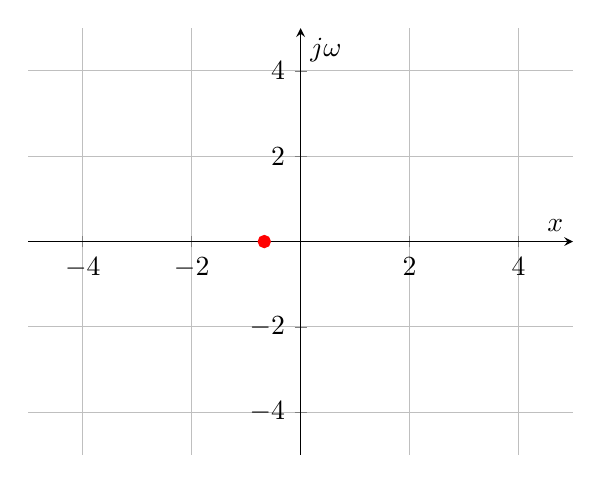
\begin{tikzpicture}
    \begin{axis}[
        axis lines=middle,
        xlabel={$x$},
        ylabel={$j\omega$},  
        grid=both,
        width=8.5cm,
        height=7cm,
        ymin=-5, ymax=5,
        xmin=-5, xmax=5,
      ]
      \addplot[red, thick, mark=*] coordinates {(-2/3,0)};
    \end{axis}
  \end{tikzpicture}
\end{figure}

Para la ecuacion de segundo orden 

$$H(s) = \dfrac{\dfrac{s}{L}}{s^2 + \dfrac{R}{L} s + \dfrac{1}{LC}}$$

Y los polos se encontrarian en $s_n=\dfrac{-\dfrac{R}{L} \pm \sqrt{\dfrac{R}{L}^2-\dfrac{4}{LC}}}{2}$

Donde reemplazando con los valores previamente dados, los polos quedarian en $(-1,0)$ y $(-2,0)$.

\begin{figure}[H]
  \centering
  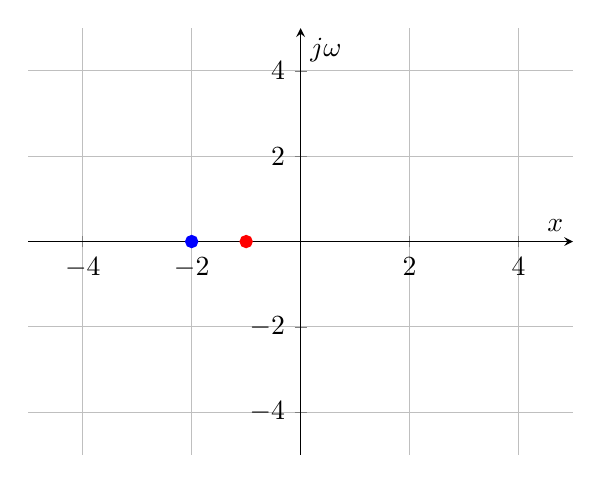
\begin{tikzpicture}
    \begin{axis}[
        axis lines=middle,
        xlabel={$x$},
        ylabel={$j\omega$},  
        grid=both,
        width=8.5cm,
        height=7cm,
        ymin=-5, ymax=5,
        xmin=-5, xmax=5,
      ]
      \addplot[red, thick, mark=*] coordinates {(-1,0)};
      \addplot[blue, thick, mark=*] coordinates{(-2,0)};
    \end{axis}
  \end{tikzpicture}
\end{figure}


\chapter{Ejercicio 3}

\section{A}

\section{B}

\chapter{Ejercicio 4}

\section{A}

\section{B}

\chapter{Ejercicio 5}

\section{A}

\section{B}

\chapter{Ejercicio 6}

\section{A}

\section{B}


\end{document}

